\documentclass{article}

\usepackage[margin=1in]{geometry}
\usepackage{amsmath,amsthm,amssymb}
\usepackage{array,multirow}
\usepackage{bbm, enumerate}
\usepackage[yyyymmdd,hhmmss]{datetime}
\usepackage{hyperref}
\usepackage{tikz}

\pgfdeclarelayer{background}   % declare background layer
\pgfsetlayers{background,main} % set the order of the layers (main is the standard layer)

\newcommand{\s}[1]{\{ #1 \}}
\renewcommand{\k}{\mathbf k}

\let\originalleft\left
\let\originalright\right
\renewcommand{\left}{\mathopen{}\mathclose\bgroup\originalleft}
\renewcommand{\right}{\aftergroup\egroup\originalright}

\newcommand{\n}[1]{\multicolumn{1}{|c|}{#1}}

\numberwithin{equation}{subsection}

\newtheorem{theo}{Theorem}[subsection]
\newtheorem{definition}[theo]{Definition}
\newtheorem{conjecture}[theo]{Conjecture}
\newtheorem{lemma}[theo]{Lemma}
\newtheorem{theorem}[theo]{Theorem}
\newtheorem{datatable}[theo]{Table}
\newtheorem{example}[theo]{Example}
\newtheorem{note}[theo]{Note}
\newtheorem{todo}[theo]{To Do}

\begin{document}

\title{Oral Exam: Proposal}
\author{Peter Kagey}

\maketitle

This document will explore two ideas for dissertation chapters in two different
sections.
The first section explores how restricting the cycle structure of a permutation
affects the expected value of its first letter. In particular, there seems to
be a hidden relationship with derangements of $n$-dimensional hypercubes and
the generalized symmetric group more broadly.
The second section generalizes a puzzle, and develops (or proves the
non-existence of) conditions under which there exists an algorithm for
a certain kind of walk reaching every element of a finite group with a random
(or an adversarial) player trying to prevent this.

\tableofcontents

\section{Expected value of the first letter of a permutation}
The genesis of this problem comes from a talk that Sami relayed to me during
which the speaker described a surprising and elegant relationship between the
number of descents in a permutation and the expected value of the first letter:
\begin{quote}
Given some $\pi \in S_n$, let $\operatorname{des}(\pi)$ give the number of
descents of $\pi$, that is \begin{equation}
  {\operatorname{des}(\pi) = \#\{i : \pi(i) > \pi(i+1)\}}.
\end{equation}

For all $n$, the expected value of $\pi(1)$ for a permutation
$\pi \in S_n$ with $k$ descents is $k+ 1$.
\end{quote}
Sami challenged me to look at other permutation statistics and to find other
relationships.
\subsection{Definitions, notation, and background}
\begin{definition}
  A \textbf{permutation statistic} is simply a map $\operatorname{st} \colon S_n \rightarrow \mathbb Z$.
\end{definition}
\begin{definition}
  Given a permutation statistic $\operatorname{st}$, let
  $\mathbb{E}_{n,m}^\text{st}$ denote the expected value of the first letter
  of a permutation taken uniformly at random from
  $\{\pi \in S_n \mid \operatorname{st}(\pi) = m\}$.
\end{definition}

\subsection{Main conjecture}
Perhaps the richest permutation statistic that I found was the three parameter
family given by looking at permutations in $S_n$ with exactly $m$ $k$-cycles.

\begin{definition}
  Let $\operatorname{cyc}_k(\pi)$ be the number of $k$-cycles in the cycle decomposition of $\pi$.
\end{definition}

\begin{conjecture}
  \label{mainConjecture}
  For $k > 1$,
  \begin{equation}
    \label{eq:mainConjecture}
    \mathbb{E}_{n,m}^{\text{cyc}_k} = \begin{cases}
      \displaystyle\frac{n+1}{2} + \frac{(-1)^{n/k-m}}{2 A320032(\frac nk - m, k)} & k \mid n \\
      \displaystyle\frac{n+1}{2} & \text{otherwise}
    \end{cases},
  \end{equation} where \href{https://oeis.org/A320032}{OEIS sequence} $A320032(n,k)$ is the number of derangements of the
  wreath product $\mathbb Z_k \wr S_n$, given by the expansion of the
  exponential generating function \begin{equation}
    \frac{\exp(-x)}{1 - kx}.
  \end{equation}
\end{conjecture}

This conjecture was suggested by computational evidence, some of which is
reflected in the following two tables.

\begin{datatable} $\mathbb{E}_{n,m}^{\text{cyc}_2}$ gives the expected value of the first letter of
  $\pi \in S_n$, given that $\pi$ has $m$ $2$-cycles.
\begin{equation}
  \begin{array}{|ll|l|l|l|l|l|l|l|}
  \hline
  & & \multicolumn{6}{|c|}{m} \\ \cline{3-8}
  & & 0 & 1 & 2 & 3 & 4 & 5 \\ \hline
  \multirow{7}{*}{$n$}
  & \n{2}  & 1/1        & 2/1      &        &      &     &     \\ \cline{2-4}
  & \n{3}  & 2/1        & 2/1      &        &      &     &     \\ \cline{2-5}
  & \n{4}  & 13/5       & 2/1      & 3/1    &      &     &     \\ \cline{2-5}
  & \n{5}  & 3/1        & 3/1      & 3/1    &      &     &     \\ \cline{2-6}
  & \n{6}  & 101/29     & 18/5     & 3/1    & 4/1  &     &     \\ \cline{2-6}
  & \n{7}  & 4/1        & 4/1      & 4/1    & 4/1  &     &     \\ \cline{2-7}
  & \n{8}  & 1049/233   & 130/29   & 23/5   & 4/1  & 5/1 &     \\ \cline{2-7}
  & \n{9}  & 5/1        & 5/1      & 5/1    & 5/1  & 5/1 &     \\ \cline{2-8}
  & \n{10} & 12809/2329 & 1282/233 & 159/29 & 28/5 & 5/1 & 6/1 \\ \hline
  \end{array}
\end{equation}
\end{datatable}
\begin{datatable} $\mathbb{E}_{n,m}^{\text{cyc}_3}$ gives the expected value of the first letter of
  $\pi \in S_n$, given that $\pi$ has $m$ $3$-cycles.
\begin{equation}
  \begin{array}{|ll|l|l|l|l|l|l|l|l|l|l|}
  \hline
  & & \multicolumn{4}{|c|}{m} \\ \cline{3-6}
  & & 0 & 1 & 2 & 3 \\ \hline
  \multirow{8}{*}{$n$}
  & \n{2} & 3/2      &        &      &      \\ \cline{2-4}
  & \n{3} & 7/4      & 5/2    &      &      \\ \cline{2-4}
  & \n{4} & 5/2      & 5/2    &      &      \\ \cline{2-4}
  & \n{5} & 3/1      & 3/1    &      &      \\ \cline{2-5}
  & \n{6} & 46/13    & 13/4   & 4/1  &      \\ \cline{2-5}
  & \n{7} & 4/1      & 4/1    & 4/1  &      \\ \cline{2-5}
  & \n{8} & 9/2      & 9/2    & 9/2  &      \\ \cline{2-6}
  & \n{9} & 1159/232 & 131/26 & 19/4 & 11/2 \\ \hline
  \end{array}
\end{equation}
\end{datatable}
\begin{note}
  As mentioned in the conjecture the "error" term in the $k \mid n$ case is
  related to the wreath product $\mathbb Z_k \wr S_n$.
  Specializing to $k = 2$, this is the hyperoctahedral group,
  so the error is related to the number of isometries of the $n$-dimensional
  hypercube that move $(n-1)$-dimensional facets.
  (I don't know how to explain this phenomenon, but I'd like to find out.)
\end{note}
\subsection{Some recurrences}
I've made some headway in proving this conjecture. In particular, I can
compute $\mathbb{E}_{n,m}^{\text{cyc}_k}$ much faster than brute force,
I have useful related recurrences, and
I have found a bijection that proves the "otherwise"
part of the conjecture.
\begin{definition}
  Let $C_k(n,m)$ be the number of permutations $\pi \in S_n$ such that
  $\operatorname{cyc}_k(\pi) = m$.
\end{definition}
\begin{definition}
  Let $C^{(\ell)}_k(n,m)$ be the number of permutations $\pi \in S_n$ such that
  $\operatorname{cyc}_k(\pi) = m$ and $\pi(1) = \ell$.
\end{definition}
\begin{lemma}
  $C_k^{(1)}(n,m) = C_k(n-1, m)$ for all $k \geq 2$.
\end{lemma}
\begin{proof}
  Writing $\pi$ as a word, consider the map
  $\pi_1\pi_2\dots\pi_n \mapsto (\pi_2 - 1)\dots(\pi_n - 1)$. Since
  $\pi_1 = 1$, the inverse map is clear.
\end{proof}
\begin{lemma}
  $C_k^{(2)}(n,m) = \cdots = C_k^{(n)}(n,m)$.
\end{lemma}
\begin{proof}
  It is enough to show that $C_k^{(a)}(n,m) = C_k^{(b)}(n,m)$ for all
  $a, b > 1$. Since the permutations under consideration do not fix $1$,
  conjugation by $(ab)$ is an isomorphism which takes all words starting
  with $a$ to words starting with $b$ without changing the cycle structure.
\end{proof}


\begin{lemma}
  \label{cyc1Recurrence}
  $C_k^{(1)}(n,m) = C_k(n-1, m)$ for all $k \geq 2$.
\end{lemma}
\begin{proof}
  Writing $\pi$ as a word, consider the map
  $\pi_1\pi_2\dots\pi_n \mapsto (\pi_2 - 1)\dots(\pi_n - 1)$. Since
  $\pi_1 = 1$, the inverse map is clear.
\end{proof}
\begin{lemma}
  \label{allSame}
  $C_k^{(2)}(n,m) = \cdots = C_k^{(n)}(n,m)$.
\end{lemma}
\begin{proof}
  It is enough to show that $C_k^{(a)}(n,m) = C_k^{(b)}(n,m)$ for all
  $a, b > 1$. Since the permutations under consideration do not fix $1$,
  conjugation by $(ab)$ is an isomorphism which takes all words starting
  with $a$ to words starting with $b$ without changing the cycle structure.
\end{proof}
\begin{lemma}
  \label{cycRecurrenceWithFixedBeginning}
  For all $2 \leq a \leq n$, \begin{align}
    C_k^{(a)}(n,m) = \frac{C_k(n, m) - C_k(n-1, m)}{n - 1}.
  \end{align}
\end{lemma}
\begin{proof}
  Since \begin{align}
    C_k(n, m) = C_k^{(1)}(n, m) + C_k^{(2)}(n, m) + \dots + C_k^{(n)}(n, m)
  \end{align} using Lemma \ref{allSame}, for all values $2 \leq a \leq n$,
  this can be rewritten as \begin{align}
    C_k(n, m) = C_k^{(1)}(n, m) + (n-1)C_k^{(a)}(n, m)
  \end{align} solving for $C_k^{(a)}(n, m)$ and using the substitution from Lemma
  \ref{cyc1Recurrence} gives the desired result: \begin{align}
    C_k^{(a)}(n, m) = \frac{C_k(n, m) - C_k(n-1, m)}{n - 1}.
  \end{align}
\end{proof}
\begin{theorem}
  \label{basecase}
  The base case, $C_k(n,0)$ is given by the expansion of the exponential
  generating function \begin{equation}
    \frac{\exp(-x^k/k)}{(1-x)},
  \end{equation} and moreover, \begin{equation}
    C_k(n,0)
    = \sum_{i=0}^{\lfloor n/k \rfloor} \frac{n! (-1)^i}{i!\,k^i}
    = A122974(n,k).
  \end{equation}
  % These appear in the OEIS as
  % \begin{align}
  %   C_1(n,0) &= A000166(n) \\
  %   C_2(n,0) &= A000266(n) \\
  %   C_3(n,0) &= A000090(n) \\
  %   C_4(n,0) &= A000138(n) \\
  %   C_5(n,0) &= A060725(n) \\
  %   C_6(n,0) &= A060726(n)
  % \end{align}
\end{theorem}
\begin{proof}
  A probabilistic proof can be found here.
  \url{http://capone.mtsu.edu/dwalsh/NOKCYCLB.pdf}
\end{proof}
\begin{note}
  I'd like to find a combinatorial proof of this fact, and I'd like to see if
  I can modify the probabilistic proof to prove Conjecture \ref{mainConjecture}.
\end{note}
% \begin{todo}
%   I'd like to find a combinatorial proof.
% \end{todo}
\begin{theorem}
  \label{cycRecurrence}
  For all $k > 0, m > 0$ \begin{equation}
    mC_k(n, m) = (k-1)!\binom{n}{k}C_k(n-k, m-1).
  \end{equation}
\end{theorem}
\begin{proof}
  As an abuse of notation, let $C_k(n, m) = \{ \pi \in S_n \mid \operatorname{cyc}_k(\pi) = m\}$.
  Then consider the two sets, whose cardinalities match the left- and
  right-hand sides of the equation above:
  \begin{align}
    S^{L}_{n,m,k} &= \{ (\pi, c) \mid \pi \in C_k(n, m), c \text{ a distinguished } k\text{-cycle of } \pi \} \\
    S^{R}_{n,m,k} &= \{ (\sigma, d) \mid \pi \in C_k(n-m, m-1), d \text{ an } n\text{-ary necklace of length } k\}
  \end{align}
  The first set, $S^{L}_{n,m,k}$, is constructed by taking a permutation in
  $C_k(n,m)$ and choosing one of its $m$ $k$-cycles to be distinguished, so
  $S^{L}_{n,m,k} = mC_k(n,m)$.

  In second set, $S^{R}_{n,m,k}$, the two parts of the tuple are independent.
  There are $C_k(n-k, m-1)$ choices for $\sigma$ and $(k-1)!\binom{n}{k}$
  choices for $d$. Thus $S^{R}_{n,m,k} = (k-1)!\binom{n}{k}C_k(n-k, m-1)$.

  Now, consider the map $\phi \colon S^{L}_{n,m,k} \rightarrow S^{R}_{n,m,k}$
  which in cycle notation does the following \begin{equation}
    (\pi_1\pi_2 \dots \pi_\ell, \pi_1) \mapsto (\pi'_2 \dots \pi'_\ell, \pi_1)
  \end{equation} where $\pi'_i$ is $\pi_i$ after relabeling.

  By construction, $\sigma$ has one fewer $k$-cycle and $k$ fewer letters
  than $\pi$.
\end{proof}
\begin{example}
  Suppose $\pi = (18)\mathbf{(37)}(254)$ in cycle notation with $(37)$ distinguished.
  Then \begin{align}
    ((18)(37)(254), (37)) \mapsto ((16)(243), (37))
  \end{align} under this bijection.
\end{example}
\begin{theorem}
  \label{expectedValueCyck}
  For $k > 1$, the expected value of the first letter of a permutation
  $\pi \in S_n$ with $m$ $k$-cycles is given by \begin{align}
    E_{n,m}^{\text{cyc}_k} = \frac n2\left(1 - \frac{C_k(n-1,m)}{C_k(n,m)}\right) + 1.
  \end{align}
\end{theorem}
\begin{proof}
  By definition, \begin{align}
    E_{n,m}^{\text{cyc}_k} = \frac{
      \displaystyle \sum_{a = 1}^n aC_k^{(a)}(n, m)
    }{
      C_k(n, m)
    }.
  \end{align} Using Lemma \ref{allSame}, we can consolidate all but the first term of
  the numerator \begin{align}
    \sum_{a = 1}^n aC_k^{(a)}(n, m) &=
    C_k^{(1)}(n,m) + \sum_{a = 2}^n aC_k^{(n)}(n, m) \\
    &= C_k^{(1)}(n,m) + C_k^{(n)}(n, m)\sum_{a = 2}^n a \\
    &= C_k^{(1)}(n,m) + \frac{(n-1)(n+2)}{2} C_k^{(n)}(n, m) \\
  \end{align}
  Now using the recurrences in Lemmas \ref{cyc1Recurrence} and
  \ref{cycRecurrenceWithFixedBeginning} \begin{align}
    \sum_{a = 1}^n aC_k^{(a)}(n, m) &=
    C_k(n-1,m) + \frac{(n-1)(n+2)}{2}\left(
      \frac{C_k(n, m) - C_k(n-1, m)}{n - 1}
    \right) \\
    &= \left(\frac{n}{2} + 1\right) C_k(n,m) - \frac n2C_k(n-1,m).
  \end{align}
  Lastly, dividing by the numerator yields the result \begin{align}
    E_{n,m}^{\text{cyc}_k}
    = \frac{
      \left(\frac{n}{2} + 1\right) C_k(n,m) - \frac n2C_k(n-1,m)
    }{
      C_k(n, m)
    }
    = \frac n2\left(1 - \frac{C_k(n-1,m)}{C_k(n,m)}\right) + 1.
  \end{align}
\end{proof}
% \begin{todo}
%   Why does this proof fail when $k = 1$?
% \end{todo}
\begin{note}
  Theorem \ref{expectedValueCyck} together with Theorem \ref{basecase} and
  Theorem \ref{cycRecurrence} give a computationally inexpensive way to
  compute $\mathbb{E}_{n,m}^{\text{cyc}_k}$.
\end{note}

\subsection{A bijective proof}
One plausible proof strategy is based on Theorem \ref{expectedValueCyck},
namely making sense of the ratio $\frac{C_k(n-1,m)}{C_k(n,m)}$. In particular,
to show the ``$k \nmid n$'' case of Conjecture \ref{mainConjecture}, it is
enough to show that the ratio is equal to $n$, or equivalently, that
$nC_k(n-1,m) = C_k(n,m)$.

The nicest combinatorial proof of this fact would be a family of bijections
$\varphi_k \colon [n] \times S_{n-1} \rightarrow S_n$ that preserves the
number of $k$ cycles when $k \nmid n$.

\begin{note}
  No such map can exist when $k \mid n$ because in that case there exist
  permutations in $S_n$ consisting of $n/k$ disjoint $k$-cycles, but no
  permutation in $S_{n-1}$ can contain this many $k$-cycles.
\end{note}

\begin{theorem}
  \label{bijection}
  The exists a bijective map
  $\varphi_k \colon [n] \times S_{n-1} \rightarrow S_n$ that preserves
  $k$-cycles when $k \nmid n$.
\end{theorem}
\begin{proof}
  I will construct such a map and the inverse of such a map. The bijection is
  easy to implement but more difficult to write down. It will be clear
  from the construction that it preserves the number of $k$-cycles.
  In this section, the names of the arguments and output of the function will
  follow the convention $\varphi_k(i, \pi) = \pi'$, where $\pi$ has cycles
  $c_1 c_2 \dots c_N$. (And $\pi'$ has cycles $c_1' c_2' \dots c_{N'}'$.)
  The cycles themselves have letters $c_i = (c_{i,1} c_{i,2} \dots c_{i,d_i})$,
  where $c_{i,d_i + 1} = c_{i,1}$.
  Moreover the letters of each cycle chosen so that the smallest letter is first,
  after which the cycles are written in lexicographic order.

  \begin{itemize}
    \item The permutation $\pi'$ sends $1 \mapsto i$.
    \item If the cycle that $1$ is in is called the \textit{initial cycle},
      then if $\pi$ has an initial $\ell$ cycle then \begin{itemize}
        \item If $i = 1$, then $c_1' = (1)$,
        \item if $|c_1| = k$, then $|c_1'| = k$,
        \item if $|c_1| = k-1$ then $|c_1'| = k + 1$,
        \item otherwise, $|c_1'| = |c_1| + 1$.
      \end{itemize}
  \end{itemize}

  These are choices so that the inverse map can recover the ``added'' letter and
  so that the combinatorics works.

  (For the sake of simplicity, when describing the behavior of $\varphi_k$,
  assume that the arguments are normalized so that the letters are $[N]$, with
  the first argument being considered smaller in the case of a tie.
  For example, instead of talking about $\phi_k(3, (25)(93))$, I'll instead
  describe $\phi_k(2, (14)(53))$.)

  \begin{itemize}
    \item When $i = 1$, $\phi_k$ simply adds a
    $1$-cycle to $\pi$: in cycle notation, $\pi' = (1)\pi$.
    \item When the $c_1 > k$ or $c_1 < k -1$, $\phi_k$ inserts $i$ after $1$
    in the cycle.
    (e.g. $\phi_2(4,(1726)(53))= (14726)(53)$.)
    \item When $|c_1| = k$, $\pi' = (c_{1,1}ic_{1,3}\dots c_{1,d_1})\phi_k(c_{1,2},c_2\dots c_N)$.
    (e.g $\phi_2(4,(17)(2653)) = (14) \phi_2(7, (2653))$.)
    \item The bijection is most complex when $|c_1| = k - 1$.
  \end{itemize}
  When $|c_1| = k - 1$, you ``insert $i$ and take from the next cycle''. The
  ``take from the next cycle'' requires and auxillary function $\psi_k$ which
  takes a $(k-1)$-cycle and a permutation and returns a permutation. \begin{equation}
    \psi_k((\alpha_1 \alpha_2 \dots \alpha_{k-1}), \pi) = \begin{cases}
      (\alpha_1 c_{1,1} \alpha_2 \dots \alpha_{k-1})c_2 \dots c_N & |c_1| = 1 \\
      (\alpha_1 c_{1,2} \alpha_2 \dots \alpha_{k-1})\psi_k((c_{1,1}c_{1,3} \dots c_{1,k}), c_2 \dots c_N) & |c_1| = k \\
      (\alpha_1 c_{1,2} \alpha_2 \dots \alpha_{k-1})(c_{1,1}c_{1,3}\dots c_{1,d_1})c_2 \dots c_N & \text{otherwise}
    \end{cases}.
  \end{equation}
  Thus when $|c_1| = k-1$, \begin{equation}
    \varphi_k(i, \pi) = \begin{cases}
      (c_{1,1} i c_{2,1} c_{1,2} \dots c_{1,k-1}) c_3 \dots c_N & |c_2| = 1 \\
      (c_{1,1} i c_{2,2} c_{1,2} \dots c_{1,k-1})\psi_k((c_{2,1} c_{2,3}\dots c_{2,k}), c_3 \dots c_N) & |c_2| = k \\
      (c_{1,1} i c_{2,2} c_{1,2} \dots c_{1,k-1})(c_{2,1})(c_{2,3}\dots c_{2,k+1}) c_3 \dots c_N & |c_2| = k+1 \\
      (c_{1,1} i c_{2,2} c_{1,2} \dots c_{1,k-1})(c_{2,1} c_{2,3}\dots c_{2,d_2}) c_3 \dots c_N & \text{otherwise} \\
    \end{cases}.
  \end{equation}
\end{proof}
This bijection $\varphi_k$ preserves the number of $k$-cycles when
$k \nmid n$, but can sometimes fail to preserve $k$-cycles when $k \mid n$,
as explored in the next section.

\subsection{Generating function}
Theorem \ref{bijection} takes care of the case where $k \nmid n$, but an
analysis of where the bijection fails to preserve the number of $k$-cycles does
not easily yield Conjecture \ref{mainConjecture}.

I'm most interested in the case where $k = 2$, and moreover my previous results
for this case have generalized easily to $k > 2$, so for the remainder of this
section, I'll specialize to $k = 2$.

\begin{definition}
  Let the failure of the bijection to preserve $k$-cycles be measured by the
  function \begin{equation}
    \operatorname{Error}_k(n,m) := C_k(n,m) - nC_k(n-1,m).
  \end{equation}
\end{definition}

\begin{conjecture}
  \label{errorConjecture}
  When $k = 2$ it appears that \begin{align}
    \operatorname{Error}_2(2n,m) &= (-1)^{n + m + 1}(2n - 1)!!\left(\binom{n-1}{m}\binom{n-1}{m-1}\right) \\
    \operatorname{Error}_2(2n + 1,m) &= 0
  \end{align}
  where $(2n-1)!! = (2n-1) \cdot (2n-3) \cdots 5 \cdot 3 \cdot 1$.
\end{conjecture}

My next steps for this project involve taking Conjecture \ref{errorConjecture}
for granted and solving for $A320032$ in Equation \ref{eq:mainConjecture}, seeing
if temporarily assuming the conjecture, using generating function tricks,
and working backward is a viable proof strategy.

In particular, I'd like to prove \begin{align}
  \mathbb{E}_{n,m}^{\text{cyc}_2}
  &= n\left(1 - \frac{C_2(2n - 1, m)}{C_2(2n, m)}\right) + 1 \label{eq:1}\\
  &= \frac{2n+1}{2} + \frac{(-1)^{n-m}}{2 A320032(n - m, 2)} \label{eq:2}
\end{align} where Equation \ref{eq:1} follows from Theorem \ref{expectedValueCyck},
and Equation \ref{eq:2} is Conjecture \ref{mainConjecture}.
Solving for $C_2(2n-1,m)$ gives \begin{equation}
  C_2(2n-1,m) = \frac{C_2(2n, m) + (-1)^{n + m}(2n - 1)!!\left(\binom{n-1}{m}\binom{n-1}{m-1}\right)}{2n},
\end{equation}
so taking Conjecture \ref{errorConjecture} for granted, means that proving
Conjecture \ref{mainConjecture} is equivalent to showing that \begin{equation}
  \frac{2n+1}{2} + \frac{(-1)^{n-m}}{2 A320032(n - m, 2)} = n\left(1 - \frac{C_2(2n, m) + (-1)^{n + m}(2n - 1)!!\left(\binom{n-1}{m}\binom{n-1}{m-1}\right)}{2nC_2(2n, m)}\right) + 1.
  \label{eq:errorSubstitution}
\end{equation}
If I haven't made any mistakes, solving for $A320032$ gives
\begin{equation}
  A320032(n - m, 2) = -\frac{C_2(2n, m)}{(2n - 1)!!\left(\binom{n-1}{m}\binom{n-1}{m-1}\right)},
\end{equation}
which is a surprisingly simple rearrangment of
Equation \ref{eq:errorSubstitution} above. Since I know several recurrences for
$C_k(n, m)$, I have some hope of being able to solve this with generating
function tricks.
% in this
% expression, and see if I can get the other side to satisfy the defining E.g.f for $A320032$.

\subsection{Next steps}
There are a few different things I'd like to explore next. \begin{itemize}
  \item I have a document with tables of other permutation statistics.
    Some of these don't look like they have much structure, but some of them
    might be amenable to this sort of analysis.
  \item I'm interested in specifying more data about the cycle structure. For example,
    \begin{itemize}
      \item If the cycle structure is fully specified by a partition of $n$.
      \item If the cycle structure is partly specified (e.g. $\pi$ has exactly three fixed points and one transposition.)
    \end{itemize}
  \item I'd like to make the connection to derangements of wreath products, and
  to derangements of the hyperoctahedral group in particular.
  (This is the case where $k = 2$).
  \item It appears that \begin{equation}
      nC_k(kn-1, m-1) = mC_k(kn, m)
    \end{equation} and it would be nice to have a combinatorial proof for why.
  \item I'd like to prove (or disprove) that \begin{equation}
      C_k(kn, i) + C_k(kn, k-i) = kn\left(C_k(kn-1, i) + C_k(kn-1, k-i)\right)
    \end{equation} and in particular when $i = 0$, \begin{equation}
      C_k(kn, 0) - knC_k(kn-1, 0) = C_k(kn, k).
    \end{equation}
\end{itemize}
\pagebreak
\section{Spinning Switches}
The second problem is inspired by a puzzle that came up at the
2019 Graduate Student Combinatorics Conference in Philadelphia.
I first saw the puzzle in
\href{https://mathriddles.williams.edu/?p=77}{Steve Miller's Math Riddles}
collection, I introduced the puzzle to a few attendees of the 2019 GSCC, and
after a few days we were able to generalize the puzzle somewhat.
It turns out that both the puzzle and the generalization that we found was
in Peter Winkler's \textit{Mathematical Puzzles: A Connoisseur's Collection}:
\begin{quote}
  Four identical, unlabeled switches are wired in series to a light bulb.
  The switches are simple buttons whose state cannot be directly observed,
  but can be changed by pushing; they are mounted on the corners of a rotatable
  square. At any point, you may push, simultaneously, any subset of the buttons,
  but then an adversary spins the square. Show that there is a deterministic
  algorithm that will enable you to turn on the bulb in at most some fixed
  number of steps.
\end{quote}
(The generalization that we found and that exists in the book is that there
also exists an algorithm for any rotating $2^n$-gon.)

\subsection{Definitions and notation}
The language that I use to generalize this puzzle is the language of wreath
products, which came up in the above section in Conjecture \ref{mainConjecture}
where the number of derangements of the generalized symmetric group
($\mathbb Z_k \wr S_n$) played a role in the error term. In the first section,
you could get away without knowing what a wreath product is, but in this section
it plays a more pivotal role. I'm defining \textit{finite} wreath products
because that's all we need, and it sidesteps some technical details.
\begin{definition}
  Let $G$ and $H$ be finite groups, and let $\Omega$ be a finite set with an $H$ action.
  Next, define $K = \prod_{\omega \in \Omega} A_\omega$ (called the \textbf{base} of the wreath product) be the
  $|\Omega|$-fold product of $G$, indexed by elements of $\Omega$.
  The $H$-action extends to $K$ by $h \cdot \alpha_\omega = \alpha_{h^{-1} \cdot \omega}$
  Then $G \wr_\Omega H$ is the semidirect product $K \rtimes H$ where
  the group multiplication is \begin{equation}
    (k_1, h_1) (k_2, h_2) = (k_1 (h_1 \cdot k_2) ,h_2 h_2).
  \end{equation}
\end{definition}

\subsection{Generalization}
I'm interested in determining criteria for when two finite groups $G$ and $H$
(together with a set $\Omega$ upon which $H$ acts) have what I call a
``switching strategy'', which in terms of the above puzzle means that there
is a deterministic finite algorithm that can turn on the bulb.

\begin{definition}
  Let $p \colon G \wr_\Omega H \rightarrow K$ be the projection map from the
  wreath product onto its base.
  A \textbf{switching strategy} is a finite sequence, $\{k_i \in K\}_{i=1}^N$,
  such that for every sequence ${\{h_i \in H\}_{i=1}^N}$,
  \begin{equation}
    p(\{e_{G \wr H}, (k_1, h_1), (k_1, h_1)\cdot(k_2, h_2), \cdots, (k_1, h_1)\cdot(k_2, h_2)\cdots(k_N, h_N)\}) = K.
  \end{equation}
\end{definition}
\begin{definition}
  A switching strategy is called \textbf{minimal} when $N = |K| - 1$.
\end{definition}

\subsection{Motivating examples.}
\begin{example}
  \label{canonicalSwitchExample}
  In the introductory example, $G = \mathbb Z_2$, $H = C_4$, and $\Omega$ is the
  vertices of a square, with $H$ acting on $\Omega$ by rotation.
  Up to the action of $H$ and the toggling of all of the switches, there are
  four distinct moves: \begin{itemize}
    \item $k_a = (1,1,1,1)$, toggling all of the switches,
    \item $k_b = (0,0,0,1)$, toggling just one of the switches,
    \item $k_c = (0,0,1,1)$, toggling two adjacent switches,
    \item $k_d = (0,1,0,1)$, toggling diagonally opposite switches.
  \end{itemize}
  Then one solution is the fifteen move sequence \begin{equation}
    k_a, k_b, k_a, k_c, k_a, k_b, k_a, k_d, k_a, k_b, k_a, k_c, k_a, k_b, k_a.
  \end{equation}
\end{example}
\begin{note}
  The exact same strategy works if Example \ref{canonicalSwitchExample} is
  modified so that $H = D_4$ the dihedral group of the square.
\end{note}
\begin{example}
  If $G = \mathbb Z_3$ and $H = C_3$, there are four possible moves up to
  toggling all switches and $H$-action:
  \begin{equation}
    \underbrace{
      \begin{tikzpicture}
        \draw (0,0) -- (1,0) -- (0.5, {sqrt(3)/2}) -- cycle;
        \node[fill=white, circle] at (0,0) {$1$};
        \node[fill=white, circle] at (0.5, {sqrt(3)/2}) {$1$};
        \node[fill=white, circle] at (1,0) {$1$};
      \end{tikzpicture}
    }_{x}
    ~
    \underbrace{
      \begin{tikzpicture}
        \draw (0,0) -- (1,0) -- (0.5, {sqrt(3)/2}) -- cycle;
        \node[fill=white, circle] at (0,0) {$0$};
        \node[fill=white, circle] at (0.5, {sqrt(3)/2}) {$1$};
        \node[fill=white, circle] at (1,0) {$0$};
      \end{tikzpicture}
    }_{A}
    ~
    \underbrace{
      \begin{tikzpicture}
        \draw (0,0) -- (1,0) -- (0.5, {sqrt(3)/2}) -- cycle;
        \node[fill=white, circle] at (0,0) {$1$};
        \node[fill=white, circle] at (0.5, {sqrt(3)/2}) {$0$};
        \node[fill=white, circle] at (1,0) {$1$};
      \end{tikzpicture}
    }_{B}
    ~
    \underbrace{
      \begin{tikzpicture}
        \draw (0,0) -- (1,0) -- (0.5, {sqrt(3)/2}) -- cycle;
        \node[fill=white, circle] at (0,0) {$1$};
        \node[fill=white, circle] at (0.5, {sqrt(3)/2}) {$0$};
        \node[fill=white, circle] at (1,0) {$2$};
      \end{tikzpicture}
    }_{C}
    ~
    \underbrace{
      \begin{tikzpicture}
        \draw (0,0) -- (1,0) -- (0.5, {sqrt(3)/2}) -- cycle;
        \node[fill=white, circle] at (0,0) {$2$};
        \node[fill=white, circle] at (0.5, {sqrt(3)/2}) {$0$};
        \node[fill=white, circle] at (1,0) {$1$};
      \end{tikzpicture}
    }_{D}
  \end{equation}
  By looking at the multiplication table in Figure \ref{multiplicationTable},
  you can create the directed graph in Figure \ref{fig:c3c3strategygraph}.
  If $x$ denotes flipping all of the switches once, then one valid strategy is
  $((x^2C)^2x^2A)^2(x^2C)^2x^2$. This is the "top" strategy in the graph.
  \begin{figure}[ht!]
    \[
      \begin{tabular}{|c|c|c|c|c|}
        \hline
          &    A      & B         &    C          &    D        \\ \hline
        A & $\s{B}$   & $\s{C,D}$ & $\s{A}$       & $\s{A}$     \\ \hline
        B & $\s{C,D}$ & $\s{A}$   & $\s{B}$       & $\s{B}$     \\ \hline
        C & $\s{A}$   & $\s{B}$   & $\s{D}$       & $\emptyset$ \\ \hline
        D & $\s{A}$   & $\s{B}$   & $\emptyset$   & $\s{C}$     \\ \hline
      \end{tabular}
    \]
  \caption{Multiplication table for states/moves in $K$ modulo rotations and
  toggling all switches.}
  \label{multiplicationTable}
  \end{figure}
  \begin{figure}[ht!]
  \center
  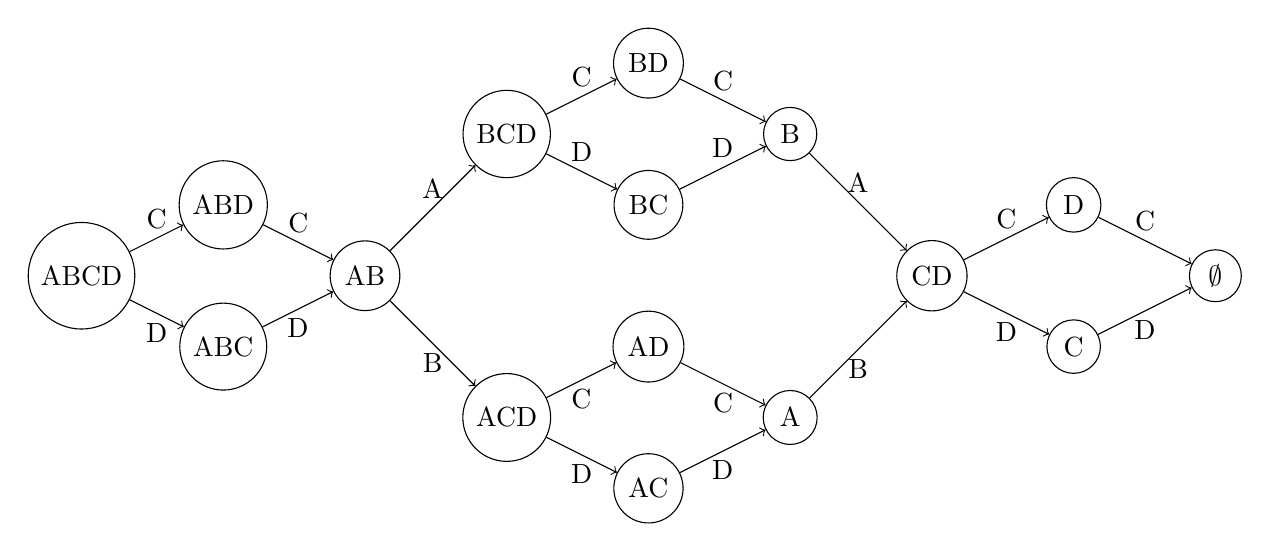
\begin{tikzpicture}[scale=0.9]
    \node[fill=white, draw, circle] (ABCD) at (0,0) {ABCD};

    \node[fill=white, draw, circle] (ABD) at (2,1) {ABD};
    \node[fill=white, draw, circle] (ABC) at (2,-1) {ABC};
    \draw (ABCD) edge[->] node[above] {C} (ABD);
    \draw (ABCD) edge[->] node[below] {D} (ABC);

    \node[fill=white, draw, circle] (AB) at (4,0) {AB};
    \draw (ABD) edge[->] node[above] {C} (AB);
    \draw (ABC) edge[->] node[below] {D} (AB);

    \node[fill=white, draw, circle] (BCD) at (6,2) {BCD};
    \node[fill=white, draw, circle] (ACD) at (6,-2) {ACD};
    \draw (AB) edge[->] node[above] {A} (BCD);
    \draw (AB) edge[->] node[below] {B} (ACD);

    \node[fill=white, draw, circle] (BD) at (8,3) {BD};
    \node[fill=white, draw, circle] (BC) at (8,1) {BC};
    \node[fill=white, draw, circle] (AD) at (8,-1) {AD};
    \node[fill=white, draw, circle] (AC) at (8,-3) {AC};
    \draw (BCD) edge[->] node[above] {C} (BD);
    \draw (BCD) edge[->] node[above] {D} (BC);
    \draw (ACD) edge[->] node[below] {C} (AD);
    \draw (ACD) edge[->] node[below] {D} (AC);

    \node[fill=white, draw, circle] (B) at (10,2) {B};
    \node[fill=white, draw, circle] (A) at (10,-2) {A};
    \draw (BD) edge[->] node[above] {C} (B);
    \draw (BC) edge[->] node[above] {D} (B);
    \draw (AD) edge[->] node[below] {C} (A);
    \draw (AC) edge[->] node[below] {D} (A);

    \node[fill=white, draw, circle] (CD) at (12,0) {CD};
    \draw (B) edge[->] node[above] {A} (CD);
    \draw (A) edge[->] node[below] {B} (CD);

    \node[fill=white, draw, circle] (D) at (14,1) {D};
    \node[fill=white, draw, circle] (C) at (14,-1) {C};
    \draw (CD) edge[->] node[above] {C} (D);
    \draw (CD) edge[->] node[below] {D} (C);

    \node[fill=white, draw, circle] (emptyset) at (16,0) {$\emptyset$};
    \draw (D) edge[->] node[above] {C} (emptyset);
    \draw (C) edge[->] node[below] {D} (emptyset);
  \end{tikzpicture}
  \caption{Switching strategy for $C_3 \wr C_3$.
  Notice that this diagram is $180^\circ$ antisymmetric:
  flipping the picture around sends sets to their complements and
  moves to their inverses.}
  \label{fig:c3c3strategygraph}
  \end{figure}
\end{example}

\begin{example}
  So far, $G$ has always been abelian, so it's worth including an example where
  $G$ is not abelian.
  Suppose that $G = D_8$, $H = \mathbb Z_2$ and $\Omega$ is a two element set
  upon which $H$ acts non-trivially. Then using the following four moves: \begin{itemize}
    \item $A_r$: Apply $r$ to both copies.
    \item $A_f$: Apply $f$ to both copies.
    \item $B$: Apply $r$ to one copy.
    \item $C$: Apply $r^2$ to one copy.
    \item $D$: Apply $f$ to one copy.
  \end{itemize}
  A strategy is $(A_r^3A_fA_r^3)B(A_r^3A_fA_r^3)C(A_r^3A_fA_r^3)B(A_r^3A_fA_r^3)D(A_r^3A_fA_r^3)B(A_r^3A_fA_r^3)C(A_r^3A_fA_r^3)B(A_r^3A_fA_r^3)$
  or if $x = A_r^3A_fA_r^3$ then the same strategy is
  $xBxCxBxDxBxCxBx$
\end{example}
\subsection{Conjectures}
\begin{conjecture}
  $\s{k_i}_{i=1}^n$ is a switching strategy if and only if $\s{k_{n-i+1}}_{i=1}^n$ is a switching strategy.
\end{conjecture}
\begin{conjecture}
  $\s{k_i}_{i=1}^n$ is a switching strategy if and only if $\s{k^{-1}_i}_{i=1}^{|K|}$ is a switching strategy.
\end{conjecture}
\begin{conjecture}
  If there exists a strategy $\s{k_i}_{i=1}^n$, then there also exists a minimal strategy $\s{k'_i}_{i=1}^{|K|}$.
\end{conjecture}
\subsection{Reduction}
For some given $G$ and $H$, there is a method to prove that no strategy exists,
which I am calling \textbf{reduction} as an allusion to the notion of reduction
in complexity theory. The idea is to show that there if there exists a strategy
that strategy can be repurposed to solve a $G'$ and $H'$ that is known to have
no solution.
For example, when $G' = \mathbb Z_2$ and $H' = C_3$, there is no strategy
because one could get stuck in a state where exactly one switch is in a
different state than the other two. This means that there is also no
strategy for $G = \mathbb Z_3$ and $H = C_6$, because if there were a switching
strategy, you could ``ignore'' every other switch and come up with a switching
strategy on $\mathbb Z_3 \wr C_3$.

More precisely, there exists a reduction from $G \wr H$ to $G' \wr H'$ if
$H'$ is isomorphic to a subset of $H$ and if there exists a quotient group of
$G$ that is isomorphic to $G'$.

There are some additional details and hypothesis here, including how the
$H$- and $H'$-actions relate to each other.
This is something that I'm still trying to make sense of.
\subsection{Next steps}
There are a few different things I'd like to explore next. \begin{itemize}
  \item I still need to prove that a $n$-gon does not have a strategy with
  $p^k$-way switches unless $n$ is a power of $p$. (I can prove the converse.)
  \item I have a very loose conjecture that given a transitive group action
  (and maybe some other natural conditions), $G \wr H$ has a switching strategy
  if and only if the cardinality of the wreath product, $|G \wr H|$, is a prime
  power.
  \item Concretely, I'd like to explore the case where the switches behave
  like the quaternion group (which is of order $2^3$). I already know there's a
  switching strategy for both cyclic groups and dihedral groups of order
  $2^\ell$, so the quaternion group is the smallest group not yet checked.
  \item I'd like to prove or disprove the three conjectures above.
  \item Of course $G \wr \mathbbm{1}$ has a switching strategy, but does it always have a palindromic switching strategy?
  \item I'd like to characterize the story for arbitrarily chosen $G$ and $H$,
  and I'd like to better understand what role the group action plays.
  \item I'm interested in some analog where the different ``switches'' can behave differently.
  (E.g. a triangle with a three-way switch and two two-way switches.)
  \item If there is not a (deterministic) switching strategy, is there some
  useful notion of a ``probabilistic'' switching strategy that minimizes the
  expected number of moves. (Assuming that the adversary picks the sequence
  ${h_i \in H}_{i=1}^{\infty}$ according to some known distribution.)
  \item Given the prominence of groups of prime power order, I'm curious if
  there's some vector space phenomena going on under the hood. If there is,
  I'd like to be able to see it.
\end{itemize}
\end{document}
